\documentclass{article}
\usepackage[utf8]{inputenc}
\usepackage{amsmath}  
\usepackage{graphicx}
\usepackage{caption}  
\usepackage{enumitem}
\usepackage{lipsum}   


\title{Pixel}
\author{Karol Kmita}
\date{\today}

\begin{document}
\maketitle


\section{Wprowadzenie}
To jest przykład dokumentu 

\begin{figure}[h]
    \centering
    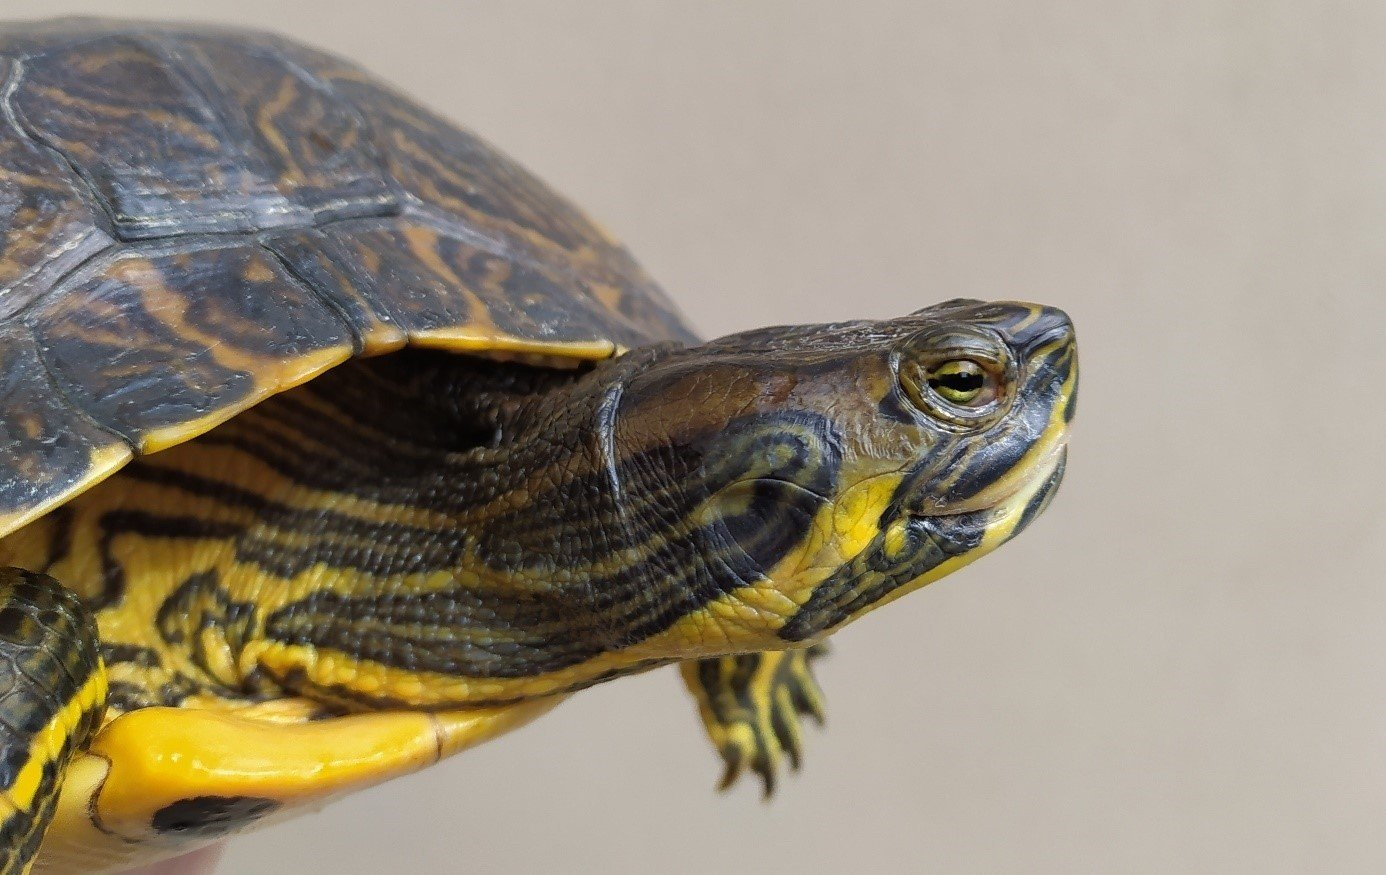
\includegraphics[width=0.7\textwidth]{pictures/zolw.jpg}
    \caption{To jest żółtolicy żółw}
    \label{fig:zolwik}
\end{figure}

Oto przykład wyrażenia matematycznego:
\begin{equation}
    x^2-y^2=(x-y)(x+y)
\end{equation}

\section{Tabela}\label{sec:tabela}

\begin{table}[h]
    \centering
    \begin{tabular}{|c|c|c|}
        \hline
        Kolumna 1 & Kolumna 2 & Kolumna 3  \\
        \hline
         Jan & 101 & zł \\
         Fran & 202 & usd \\
         Stan & 304 & euro\\
        \hline
    \end{tabular}
    \caption{jakas tabela}
\end{table}


\section{Listy}\label{sec:listy}
\begin{enumerate}
    \item Pierwsza rzezc
    \item Druga rzecz
    \item Trzecia rzecz
\end{enumerate}

\begin{itemize}
    \item iż.
    \item gdyż.
    \item ponieważ.
\end{itemize}


\textbf{Tekst pogrubiony} wystarczy użyć \texttt{\textbackslash textbf}. \emph{Tekst pochylony} Wystarczy użyć \texttt{\textbackslash emph}. W sekcji \ref{sec:tabela} znajduje się tabela, a w sekcji \ref{sec:listy} znajduje się lista. No i tak to jest.

Litwo! Ojczyzno moja! ty jesteś jak zdrowie.
Ile cię trzeba cenić, ten tylko się dowie,
Kto cię stracił. Dziś piękność twą w całej ozdobie
Widzę i opisuję, bo tęsknię po tobie.



\end{document}
